\documentclass[12pt]{article}
\usepackage{amsmath, amssymb, geometry, array, booktabs, multicol, enumitem}
\usepackage[most]{tcolorbox}
\usepackage{tikz}
\usepackage{xcolor}
\usepackage{fancyhdr}

\geometry{margin=0.85in, top=0.75in, bottom=0.9in}

%%── Palette ─────────────────────────────────────────────────────────
\definecolor{navy}{RGB}{10,36,99}
\definecolor{gold}{RGB}{195,150,30}
\definecolor{teal}{RGB}{0,120,110}
\definecolor{crimson}{RGB}{160,30,40}
\definecolor{violet}{RGB}{90,30,140}
\definecolor{midgray}{RGB}{110,110,110}
\definecolor{lightgray}{RGB}{240,240,240}
\definecolor{skyblue}{RGB}{220,235,255}
\definecolor{lightviolet}{RGB}{240,228,255}
\definecolor{lightpink}{RGB}{255,228,228}
\definecolor{lightgold}{RGB}{255,248,215}
\definecolor{lightteal}{RGB}{210,245,240}
\definecolor{ansgreen}{RGB}{20,110,40}

\tcbuselibrary{skins, breakable, theorems}

%%── Box styles ───────────────────────────────────────────────────────
\newtcolorbox{ideabox}[2]{%
  enhanced, breakable,
  colback=#1!9, colframe=#1, coltitle=white,
  fonttitle=\bfseries\large,
  title={#2},
  arc=5pt, boxrule=1.5pt,
  left=9pt, right=9pt, top=6pt, bottom=6pt,
  drop shadow={#1!35}%
}

\newtcolorbox{watchbox}{%
  enhanced,
  colback=lightpink, colframe=crimson, coltitle=white,
  fonttitle=\bfseries,
  title={$\boldsymbol{\triangleright}$ Caution --- Parentheses Matter!},
  arc=4pt, boxrule=1.3pt,
  left=8pt, right=8pt, top=5pt, bottom=5pt%
}

\newtcolorbox{pracbox}[2]{%
  enhanced, breakable,
  colback=#1!6, colframe=#1, coltitle=white,
  fonttitle=\bfseries,
  title={#2},
  arc=4pt, boxrule=1.3pt,
  left=8pt, right=8pt, top=6pt, bottom=6pt%
}

\newtcolorbox{keystrip}[1]{%
  enhanced,
  colback=#1, colframe=#1,
  arc=5pt, boxrule=0pt,
  left=10pt, right=10pt, top=7pt, bottom=7pt%
}

%%── Header / Footer ─────────────────────────────────────────────────
\pagestyle{fancy}
\fancyhf{}
\fancyhead[L]{\textcolor{navy}{\bfseries \;|\; Rational Exponents --- Practice}}
\fancyhead[R]{\textcolor{midgray}{Name:\;\underline{\hspace{4.5cm}}}}
\fancyfoot[C]{\textcolor{midgray}{\small\thepage}}
\renewcommand{\headrulewidth}{1.5pt}
\renewcommand{\headrule}{\hbox to\headwidth{\color{navy}\leaders\hrule height\headrulewidth\hfill}}

%%── Shortcuts ───────────────────────────────────────────────────────
\newcommand{\blank}{\underline{\hspace{2.8cm}}}
\newcommand{\sblank}{\underline{\hspace{1.5cm}}}
\newcommand{\lblank}{\underline{\hspace{4cm}}}

\begin{document}

%%──────────────── TITLE BANNER ──────────────────────────────────────
\begin{tcolorbox}[enhanced, arc=7pt,
  colback=navy, colframe=gold, boxrule=2.8pt,
  left=14pt, right=14pt, top=11pt, bottom=11pt]
  \begin{center}
    {\color{gold}\fontsize{22}{26}\selectfont\bfseries
      Rational Exponents --- Practice}\\[5pt]
    {\color{white}\large\itshape
      Convert $\cdot$ Simplify $\cdot$ Apply}
  \end{center}
\end{tcolorbox}

\vspace{10pt}

%%══════════════════════════════════════════════════════════════════
%%  KEY IDEAS
%%══════════════════════════════════════════════════════════════════

%%── Idea 1: Definition ─────────────────────────────────────────────
\begin{ideabox}{navy}{$\S1$ \quad Definition of Rational Exponent: $a^{1/n}$}

\textbf{Where does $a^{1/n}$ come from?} Start from something we know:
\[
2^{10} = 1024
\quad\Rightarrow\quad
(2^{10})^{\frac{1}{10}} = 1024^{\frac{1}{10}}
\quad\Rightarrow\quad
2^{10 \cdot \frac{1}{10}} = 1024^{\frac{1}{10}}
\quad\Rightarrow\quad
2 = 1024^{\frac{1}{10}}
\]

But we already know $2 = \sqrt[10]{1024}$. \; So:

\begin{center}
\begin{tcolorbox}[colback=skyblue, colframe=navy, arc=4pt, boxrule=1pt,
  left=6pt, right=6pt, top=5pt, bottom=5pt, width=0.7\linewidth]
\centering
\Large $a^{\,1/n} \;=\; \sqrt[n]{a}$
\hspace{20pt}
\normalsize ($n$th root of $a$)
\end{tcolorbox}
\end{center}

\textbf{Examples:}\quad
$9^{1/2}=\sqrt{9}=3$\hspace{1em}
$8^{1/3}=\sqrt[3]{8}=2$\hspace{1em}
$16^{1/4}=\sqrt[4]{16}=2$\hspace{1em}
$32^{1/5}=\sqrt[5]{32}=2$

\end{ideabox}

\vspace{8pt}

%%── Idea 2: General Rule ───────────────────────────────────────────
\begin{ideabox}{teal}{$\S2$ \quad General Rule: $a^{m/n}$}

When the exponent is a fraction $\dfrac{m}{n}$ (not just $\dfrac{1}{n}$), \textbf{two equivalent paths}:

\vspace{6pt}
\begin{center}
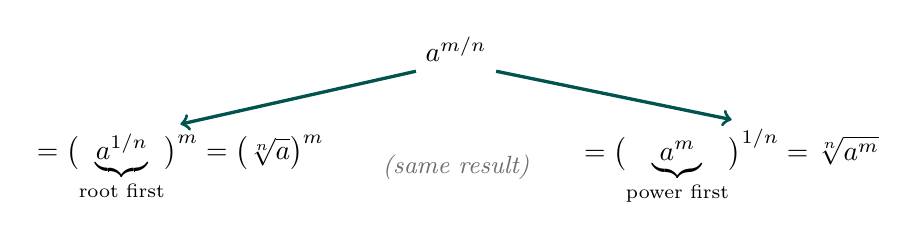
\begin{tikzpicture}[font=\normalsize, node distance=1.2cm]
  \node (start) at (0,0) {$a^{m/n}$};
  \node (pathA) at (-3.5,-1.5)
    {$= \bigl(\underbrace{a^{1/n}}_{\text{root first}}\bigr)^m
     = \bigl(\sqrt[n]{a}\bigr)^m$};
  \node (pathB) at (3.5,-1.5)
    {$= \bigl(\underbrace{a^m}_{\text{power first}}\bigr)^{1/n}
     = \sqrt[n]{a^m}$};
  \draw[->, teal!70!black, line width=1.2pt]
    (start.south west) -- (pathA.north);
  \draw[->, teal!70!black, line width=1.2pt]
    (start.south east) -- (pathB.north);
  \node[font=\small\itshape, text=midgray] at (0,-1.5)
    {(same result)};
\end{tikzpicture}
\end{center}

\vspace{4pt}
\textbf{Tip:} Root first keeps numbers small!
\hspace{1em}
$27^{4/3}$: root first $\Rightarrow (\sqrt[3]{27})^4 = 3^4 = 81$
\hspace{0.5em} vs \hspace{0.5em}
power first $\Rightarrow \sqrt[3]{27^4} = \sqrt[3]{531441} = 81$ \checkmark

\end{ideabox}

\vspace{8pt}

%%── Idea 3: Improper Fraction Exponent ────────────────────────────
\begin{ideabox}{violet}{$\S3$ \quad Improper Fraction Exponent --- Split the Whole Part}

When $m > n$ (improper fraction exponent), split off the whole number part:
\[
d^{\,5/3}
= d^{\,1 + 2/3}
= d^1 \cdot d^{\,2/3}
= d \cdot \sqrt[3]{d^2}
\]

\textbf{General strategy:}
\[
a^{\,p/q} = a^{\,\lfloor p/q \rfloor + r/q}
= a^{\,\lfloor p/q \rfloor} \cdot a^{\,r/q}
\qquad\text{where } p = \lfloor p/q\rfloor \cdot q + r
\]

\textbf{Another example:}\;
$x^{7/4} = x^{1+3/4} = x \cdot x^{3/4} = x\cdot\sqrt[4]{x^3}$

\end{ideabox}

\vspace{8pt}

%%── Caution box ────────────────────────────────────────────────────
\begin{watchbox}
\begin{multicols}{2}
\textbf{WITHOUT parentheses:}
\[
5x^{1/3} = 5\cdot\sqrt[3]{x}
\]
Only $x$ is raised to the power $\tfrac{1}{3}$.

\columnbreak

\textbf{WITH parentheses:}
\[
(5x)^{1/3} = \sqrt[3]{5x}
\]
Both $5$ and $x$ are raised to the power $\tfrac{1}{3}$.
\end{multicols}
\vspace{2pt}
\textbf{Memory trick:} the exponent only ``reaches'' what is immediately to its left.
\end{watchbox}

\vspace{8pt}

%%── Big Idea Strip ─────────────────────────────────────────────────
\begin{keystrip}{navy}
\color{white}\bfseries
Big Ideas:\quad
$a^{1/n}=\sqrt[n]{a}$
\hspace{16pt}
$a^{m/n}=(\sqrt[n]{a})^m=\sqrt[n]{a^m}$
\hspace{16pt}
Improper: split the whole part first
\end{keystrip}

\newpage

%%══════════════════════════════════════════════════════════════════
%%  PRACTICE PROBLEMS
%%══════════════════════════════════════════════════════════════════

%%── Group 1: Converting Forms ─────────────────────────────────────
\begin{pracbox}{teal}{Group 1 \quad Converting Between Forms}
\vspace{4pt}
\begin{enumerate}[label=\textbf{\arabic*.}, itemsep=18pt]

  \item Evaluate directly:\quad
        $\displaystyle(1024)^{1/10}=\sqrt[10]{1024}=\blank$

  \item Write $a^{5/6}$ in radical form:\quad $\blank$

  \item Verify both forms give the same answer for $a^{5/6}$:\quad
        $\displaystyle\bigl(\sqrt[6]{a}\bigr)^5 = \sqrt[6]{a^{\square}}
        = \blank$

  \item Rewrite with a rational exponent:\quad
        $\displaystyle\sqrt[3]{5x} = \blank$

  \item Rewrite with a rational exponent:\quad
        $\displaystyle 5\cdot\sqrt[3]{x} = \blank$
        \hfill{\small\itshape Note: different from \#4!}

  \item Convert to radical form:\quad
        $\displaystyle x^{2/5} = \blank$

  \item Convert to exponential form:\quad
        $\displaystyle\sqrt[4]{x^3} = \blank$

\end{enumerate}
\vspace{4pt}
\end{pracbox}

\vspace{10pt}

%%── Group 2: Simplify Numerical ───────────────────────────────────
\begin{pracbox}{gold}{Group 2 \quad Evaluate / Simplify (Numbers)}
\vspace{4pt}
\begin{multicols}{2}
\begin{enumerate}[label=\textbf{\arabic*.}, itemsep=20pt, start=8]

  \item $\displaystyle 8^{2/3}=\bigl(\sqrt[3]{8}\bigr)^2=\blank$

  \item $\displaystyle 27^{4/3}=\bigl(\sqrt[3]{27}\bigr)^4=\blank$

  \item $\displaystyle 16^{3/4}=\bigl(\sqrt[4]{16}\bigr)^3=\blank$

  \item $\displaystyle 64^{2/3}=\bigl(\sqrt[3]{64}\bigr)^2=\blank$

  \item $\displaystyle 81^{3/4}=\bigl(\sqrt[4]{81}\bigr)^3=\blank$

\end{enumerate}
\end{multicols}
\vspace{4pt}
\end{pracbox}

\vspace{10pt}

%%── Group 3: Simplify Algebraic ───────────────────────────────────
\begin{pracbox}{violet}{Group 3 \quad Simplify Algebraic Expressions}
\vspace{4pt}
\begin{enumerate}[label=\textbf{\arabic*.}, itemsep=18pt, start=13]

  \item $\displaystyle d^{5/3}
        = d^{1+2/3}
        = d\cdot d^{2/3}
        = d\cdot\blank$

  \item $\displaystyle\left(x^{1/2}\right)^6
        = x^{1/2\,\times\,6}
        = \blank$

  \item Rewrite with a single exponent:\quad
        $\displaystyle\sqrt[3]{\sqrt{x}}
        = \bigl(x^{1/2}\bigr)^{1/3}
        = x^{1/\square}
        = \blank$

  \item Simplify and write in radical form:\quad
        $\displaystyle\frac{x^{3/4}}{x^{1/4}}
        = x^{3/4\,-\,1/4}
        = x^{\square}
        = \blank$

  \item Simplify:\quad
        $\displaystyle\left(\frac{a^3}{a^5}\right)^4
        =(a^{3-5})^4
        =(a^{-2})^4
        = \blank$

\end{enumerate}
\vspace{4pt}
\end{pracbox}

\newpage

%%── Group 4: Applied / Prime Factorisation ────────────────────────
\begin{pracbox}{navy}{Group 4 \quad Prime Factorisation \& Multi-step}
\vspace{4pt}
\begin{enumerate}[label=\textbf{\arabic*.}, itemsep=20pt, start=18]

  \item Simplify $(54y)^{2/3}$:\quad
        \[
        (54y)^{2/3} \;=\; \blank
        \]

  \item Expand and simplify $(54y^2)^{2/3}$. \textit{Hint:}\; $54 = 2\cdot27 = 2\cdot3^3$
        \[
        (54y^2)^{2/3}
        = (2\cdot 3^3)^{2/3}\cdot y^{2/3 \cdot 2}
        = 2^{2/3}\cdot 3^{3\cdot 2/3}\cdot y^{4/3}
        = \blank
        \]

\end{enumerate}
\vspace{4pt}
\end{pracbox}

\vspace{10pt}

%%── Group 5: True/False + Challenge ──────────────────────────────
\begin{pracbox}{crimson}{Group 5 \quad True / False \& Challenge}
\vspace{4pt}
\begin{enumerate}[label=\textbf{\arabic*.}, itemsep=18pt, start=20]

  \item \textbf{True or False} --- explain your reasoning:
        \[
        4x^{1/2} \;\overset{?}{=}\; (4x)^{1/2}
        \]
        \vspace{0.2cm}
        Answer:\;\lblank

        Reason:\;\lblank

  \item \textbf{Challenge} --- simplify completely
        \textit{(apply exponent to numerator and denominator separately)}:
        \[
        \left(\frac{8x^3}{27y^6}\right)^{2/3}
        = \frac{(8x^3)^{2/3}}{(27y^6)^{2/3}}
        = \frac{8^{2/3}\cdot x^{3\cdot 2/3}}{27^{2/3}\cdot y^{6\cdot 2/3}}
        = \blank
        \]

\end{enumerate}
\vspace{4pt}
\end{pracbox}

\newpage

%%══════════════════════════════════════════════════════════════════
%%  ANSWER KEY
%%══════════════════════════════════════════════════════════════════
\begin{tcolorbox}[enhanced, arc=7pt,
  colback=navy, colframe=gold, boxrule=2.8pt,
  left=14pt, right=14pt, top=10pt, bottom=10pt]
  \begin{center}
    {\color{gold}\fontsize{18}{22}\selectfont\bfseries
      Answer Key \quad --- \quad Teacher Copy}
  \end{center}
\end{tcolorbox}

\vspace{10pt}

\begin{pracbox}{teal}{Group 1 --- Converting}
\begin{enumerate}[label=\textbf{\arabic*.}, itemsep=5pt]
  \item ${\color{ansgreen}\boldsymbol{2}}$
        \quad{\small$(2^{10}=1024 \Rightarrow 1024^{1/10}=2)$}
  \item ${\color{ansgreen}\boldsymbol{\sqrt[6]{a^5}}}$
  \item ${\color{ansgreen}\boldsymbol{\sqrt[6]{a^5}}}$ \checkmark \;both forms match
  \item ${\color{ansgreen}\boldsymbol{(5x)^{1/3}}}$
        \quad{\small(both $5$ and $x$ inside)}
  \item ${\color{ansgreen}\boldsymbol{5x^{1/3}}}$
        \quad{\small(only $x$ raised)}
  \item ${\color{ansgreen}\boldsymbol{\sqrt[5]{x^2}}}$
  \item ${\color{ansgreen}\boldsymbol{x^{3/4}}}$
\end{enumerate}
\end{pracbox}

\vspace{8pt}

\begin{pracbox}{gold}{Group 2 --- Evaluate}
\begin{multicols}{3}
\begin{enumerate}[label=\textbf{\arabic*.}, itemsep=5pt, start=8]
  \item ${\color{ansgreen}\boldsymbol{4}}$
        \;{\tiny$(\sqrt[3]{8})^2=2^2$}
  \item ${\color{ansgreen}\boldsymbol{81}}$
        \;{\tiny$(\sqrt[3]{27})^4=3^4$}
  \item ${\color{ansgreen}\boldsymbol{8}}$
        \;{\tiny$(\sqrt[4]{16})^3=2^3$}
  \item ${\color{ansgreen}\boldsymbol{16}}$
        \;{\tiny$(\sqrt[3]{64})^2=4^2$}
  \item ${\color{ansgreen}\boldsymbol{27}}$
        \;{\tiny$(\sqrt[4]{81})^3=3^3$}
\end{enumerate}
\end{multicols}
\end{pracbox}

\vspace{8pt}

\begin{pracbox}{violet}{Group 3 --- Algebraic}
\begin{enumerate}[label=\textbf{\arabic*.}, itemsep=5pt, start=13]
  \item $d\cdot{\color{ansgreen}\boldsymbol{\sqrt[3]{d^2}}}$
  \item ${\color{ansgreen}\boldsymbol{x^3}}$
        \quad{\small$\frac{1}{2}\times6=3$}
  \item $x^{{\color{ansgreen}\mathbf{1/6}}}$
        \quad{\small$(x^{1/2})^{1/3}=x^{1/6}$}
  \item $x^{{\color{ansgreen}\mathbf{1/2}}} = {\color{ansgreen}\boldsymbol{\sqrt{x}}}$
        \quad{\small$\frac{3}{4}-\frac{1}{4}=\frac{2}{4}=\frac{1}{2}$}
  \item ${\color{ansgreen}\boldsymbol{a^{-8}}}$
        \quad{\small$(a^{-2})^4=a^{-8}$}
\end{enumerate}
\end{pracbox}

\vspace{8pt}

\begin{pracbox}{navy}{Group 4 --- Prime Factorisation}
\begin{enumerate}[label=\textbf{\arabic*.}, itemsep=6pt, start=18]
  \item ${\color{ansgreen}\boldsymbol{\sqrt[3]{(54y)^2}=\sqrt[3]{2916\,y^2}}}$
  \item $2^{2/3}\cdot 3^2\cdot y^{4/3}
        = {\color{ansgreen}\boldsymbol{9\cdot\sqrt[3]{4y^4}}}
        = {\color{ansgreen}\boldsymbol{9\sqrt[3]{4}\cdot y\sqrt[3]{y}}}$
        \quad{\small$\bigl(y^{4/3}=y\cdot y^{1/3}=y\sqrt[3]{y}\bigr)$}
\end{enumerate}
\end{pracbox}

\vspace{8pt}

\begin{pracbox}{crimson}{Group 5 --- True/False \& Challenge}
\begin{enumerate}[label=\textbf{\arabic*.}, itemsep=8pt, start=20]
  \item {\color{ansgreen}\bfseries False.}\;
        $4x^{1/2}=4\sqrt{x}$ \quad but \quad
        $(4x)^{1/2}=\sqrt{4x}=2\sqrt{x}$.\;
        They differ by a factor of $2$.
  \item $\dfrac{8^{2/3}\cdot x^2}{27^{2/3}\cdot y^4}
        = \dfrac{(\sqrt[3]{8})^2\cdot x^2}{(\sqrt[3]{27})^2\cdot y^4}
        = \dfrac{4x^2}{9y^4}
        = {\color{ansgreen}\boldsymbol{\dfrac{4x^2}{9y^4}}}$
\end{enumerate}
\end{pracbox}

\end{document}
